\section{3D from Image}\label{3d from image}

The conversion of two-dimensional images into three-dimensional models represents a significant challenge in the domain of computer vision and 3D modeling. This section explores the methodologies and technologies employed in transforming 2D images into 3D models, a process that has profound implications in various fields, including virtual reality, gaming, and medical imaging. Techniques such as Magic 123 and Wonder3D will be thoroughly analyzed.

The capacity to create 3D models from images not only enhances the realism and immersion in digital experiences but also aids in practical applications like urban planning and product design. These technologies harness complex algorithms to interpret spatial information from flat images, presenting unique challenges like dealing with occlusions, varying lighting conditions, and perspective distortions

\subsection{Magic 123}\label{Magic123}

//TODO

\begin{figure}[h]
    \centering
      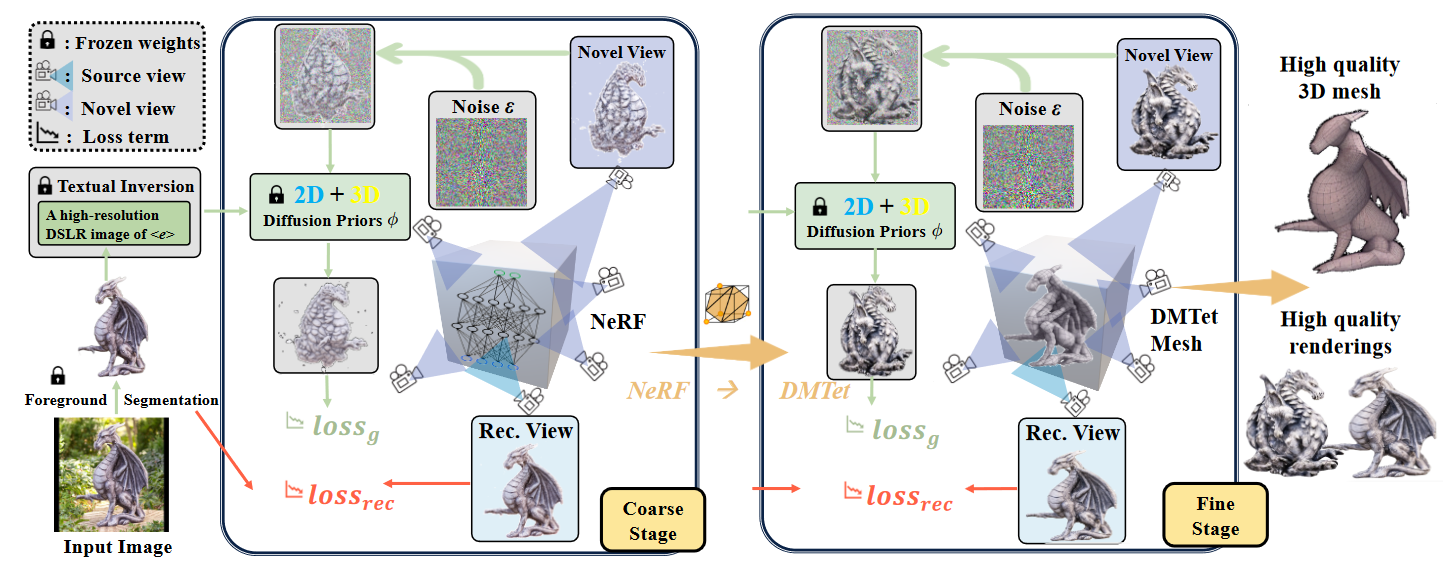
\includegraphics[width=1\columnwidth]{figures/Magic123.png}
      \caption{Summatized functionality of Magic123}\label{fig:figureMagic123}
\end{figure}
\subsection{Wonder 3D}\label{Wonder3D}

The primary innovation of Wonder3D lies in its ability to efficiently generate high-fidelity textured meshes from single images, a task that presents considerable challenges in the field of computer vision.

The method begins by generating consistent multi-view normal maps alongside corresponding color images through a cross-domain diffusion model. This process is critical for ensuring the fidelity and consistency of the generated 3D models. To achieve this, Wonder3D employs a multi-view cross-domain attention mechanism, which facilitates the exchange of information across different views and modalities, thereby enhancing the consistency and quality of the generated images \citep{long2023wonder3d}.

\begin{figure}[ht]
  \centering
    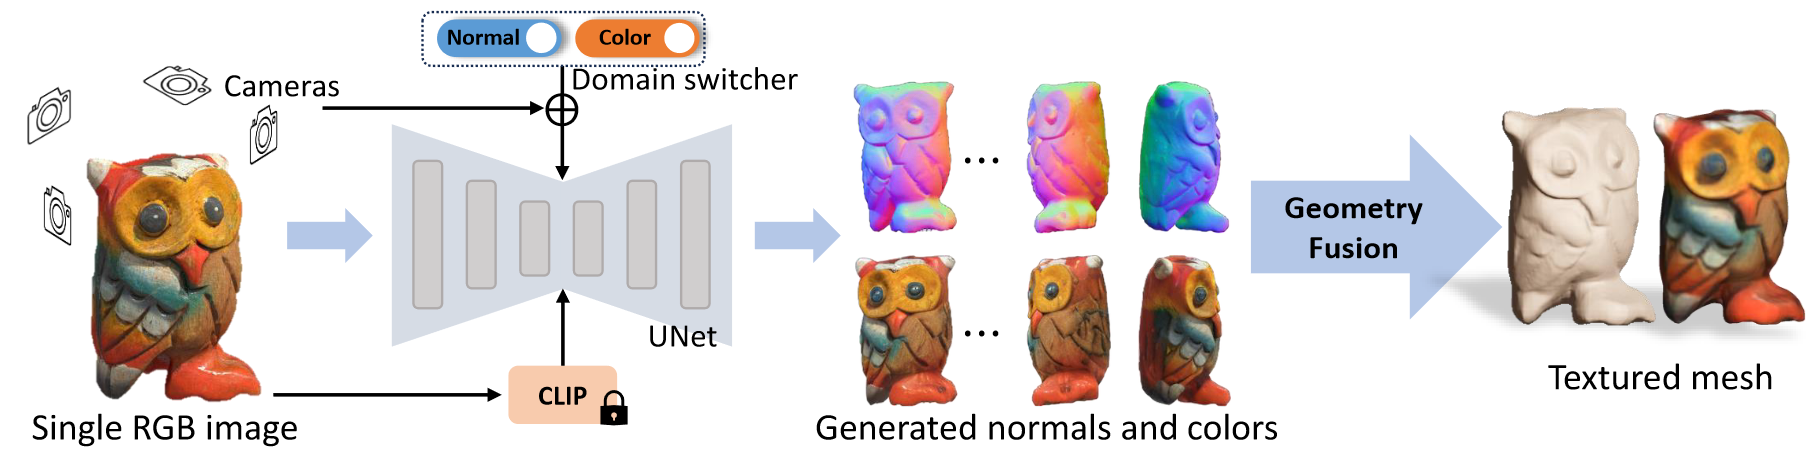
\includegraphics[width=1\columnwidth]{figures/Wonder3D.png}
    \caption{Summarized functionality of Wonder3D, depicting the method's unique approach to generating high-fidelity textured meshes from single images using cross-domain diffusion models \citep{long2023wonder3d}.}\label{fig:Wonder3D}
\end{figure}

An integral part of Wonder3D is its novel geometry-aware normal fusion algorithm. This algorithm robustly extracts high-quality surfaces from the generated multi-view 2D representations, including normal maps and color images. The fusion algorithm plays a pivotal role in reconstructing clean and detailed geometries from these 2D inputs, which is a significant step forward in the field \citep{long2023wonder3d}.

To understand this in simpler terms, imagine you have a single photo of an object, and you want to create a detailed 3D model of it. Traditional methods might struggle with this task, especially in terms of generating a model that is consistent and detailed from all angles. Wonder3D addresses this challenge by first creating multiple views of the object, as if you were looking at it from different angles. It does this by generating normal maps, which are like detailed blueprints of the object's surface textures and contours, as well as color images that match these maps. Then, using its specialized fusion algorithm, Wonder3D combines all these different views into a single, cohesive 3D model. This model not only looks good from the original angle of the photo but also from other angles, making it a more complete and accurate representation of the object.